% Style Modified from: Sharelatex, Beamer Keynote-looking style
% Which in turn came from:  www.shawnlankton.com

\documentclass[serif,mathserif]{beamer}
\usepackage{amsmath, amsfonts, epsfig, xspace}
\usepackage{algorithm,algorithmic}
\usepackage{pstricks,pst-node}
\usepackage{multimedia}
\usepackage[normal,tight,center]{subfigure}
\setlength{\subfigcapskip}{-.5em}
\usepackage{beamerthemesplit}
\usetheme{lankton-keynote}
\usepackage[absolute,overlay]{textpos}
\newcommand{\abs}[1]{\lvert#1\rvert}
\newcommand{\qi}{\text{\textbf{i}}}
\newcommand{\qj}{\text{\textbf{j}}}
\newcommand{\qk}{\text{\textbf{k}}}
\newcommand{\qq}{\text{\textbf{q}}}
\newcommand{\qr}{\text{\textbf{r}}}
\newcommand{\qu}{\text{\textbf{u}}}


\author[Sean Turner]{Sean Turner}

\title[Quaternions\hspace{2em}\insertframenumber/\inserttotalframenumber]{Rotations in 3D using Quaternions}

\date{April 21, 2017}

\institute{University of Maine, Department of Mathematics and Statistics}

\begin{document}

\maketitle

\begin{frame}
  \frametitle{Overview}
  \begin{textblock*}{2.5cm}(7.5cm,2.5cm) % {block width} (coords)
  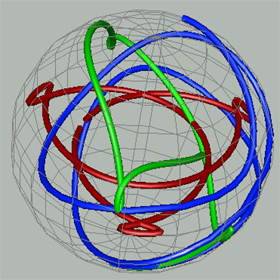
\includegraphics[width=5cm]{Images/quaternion_map.jpg}
  \end{textblock*}
 \begin{itemize}
 
  \item Introduction \& History
  \item Discussion
  \item Comparison
  \item Applications and Demonstration
  \item Questions
  \end{itemize}
\end{frame}

% \section{Main Body} % add these to see outline in slides

\begin{frame}
  \frametitle{Introduction \& History}
  \centering
  "a very curious train of mathematical speculation"
   $$ i^2 = j^2 = k^2 = ijk = -1 $$
  \begin{textblock*}{2.5cm}(4cm,5cm) % {block width} (coords)
  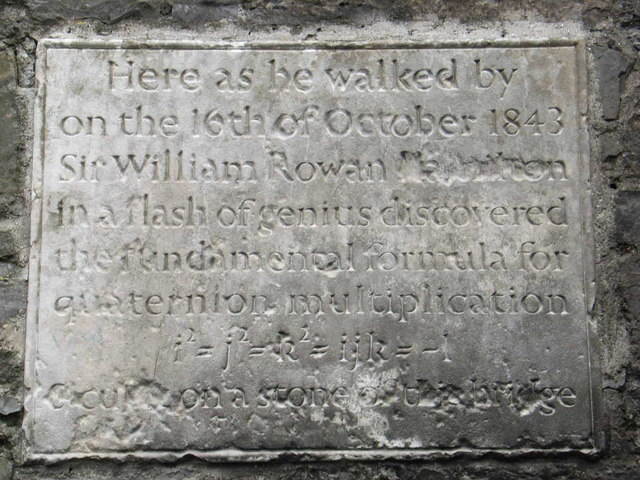
\includegraphics[width=5cm]{Images/bridge.jpg}
  \end{textblock*}
  
\end{frame}

\begin{frame} 
  \frametitle{Basic Geometric Transformations}
  \begin{itemize}
  \item 
  \textit{Translation}: A point moved from one place to another \pause
  \item \textit{Rotation}: Movement about an arbitrary axis by $\theta \in [-\pi,\pi]$.\pause
  \item Orientation vs. Rotation 
    
  \end{itemize}
\end{frame}



\begin{frame}
  \frametitle{Quaternions}
  \begin{itemize}
    \item A number in the form $a + b\qi + c\qj + d\qk $
    \begin{itemize}
        \item $i^2 = j^2 = k^2 = ijk = -1$
    \end{itemize}
    \end{itemize}
    \centering
  \vspace{0.3cm}    
      $(1 + 2\qi + 3\qj + 4\qk)$ \\
     +$(-2 + 3\qi - 1\qj + 4\qk)$\\
     =$(-1 + 5\qi + 2\qj + 8\qk)$

\end{frame}


\begin{frame}
  \frametitle{Quaternion Multiplication}
  \centering
   $\qi * \qi = -1$ \\
   $\qi\qj\qk = -1$ \\ \pause
   $\qi\qj = ? $ \\ \pause
   $\qi\qj = -\qi\qj (-1) = - \qi\qj\qk^2= -(\qi\qj\qk)\qk = -(-1)\qk = \qk $ 
\end{frame}

\begin{frame}
  \frametitle{Quaternion Multiplication Table}
  \begin{table}[H]
    \centering
    \begin{tabular}{|l|l|l|l|}
    \hline
     & \qi & \qj & \qk \\ \hline
    \qi & \text{\textbf{-1}} & \qk & -\qj \\ \hline
    \qj & -\qk & \text{\textbf{-1}} & \qi \\ \hline
    \qk & -\qj & \qi & \text{\textbf{-1}} \\ \hline
    \end{tabular}
  \end{table}
  \begin{itemize}
    \item Not Commutative! 
    \item Properties of Quaternion Multiplication:
    \begin{itemize}
      \item Associativity
      \item Distributivity
      \item Inverses
    \end{itemize}
  \end{itemize}

\end{frame}


\begin{frame}
  \frametitle{Other Quaternion Properties}
  $\qq = a + b\qi + c\qj + d\qk $
  \begin{itemize}
    \item Scalar + Vector $ \qq = S + V $
    \item \textit{Norm} $ \abs{\qq} = \sqrt{a^2 + b^2 + c^2 + d^2}.$
    \item \textit{Conjugate} $ \qq^* = S\qq - V\qq = a - b\qi - c\qj - d\qk,$
  \end{itemize}
  \vspace{0.3cm}
  Quaternions form a group
  \begin{itemize}
    \item Non-abelian $ab \neq ba$
    \item Every subgroup is normal 
    \item (\textit{Hamiltonian})
    
  \end{itemize}
\end{frame}

\begin{frame}
  \frametitle{Connecting Quaternions to Rotations}
  \textit{Theorem}: Every quaternion can be represented in the form $$ \qq =\abs{\qq}(cos(\theta) + \qu sin(\theta)) $$
  \vspace{0.3cm}
  \textit{Theorem}: Let \qr$ $ be a unit quaternion. Let R be the transformation on the pure quaternion \qq$ $ defined by $$ \text{R}\qq = \qr \qq \qr^*.$$
Then R is a rotation of the three dimensional space of pure quaternions about an axis passing through the origin.

\end{frame}

\begin{frame}
  \frametitle{Euler Angles}
  \begin{textblock*}{3cm}(6cm,5cm) % {block width} (coords)
  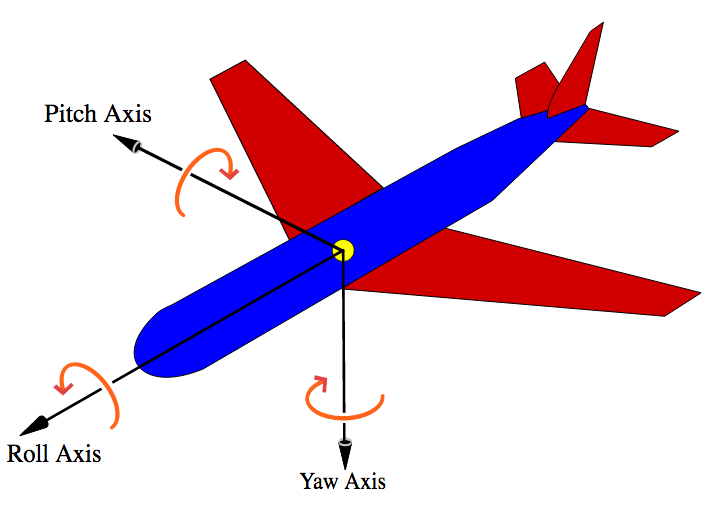
\includegraphics[width=5cm]{Images/plane.png}
  \end{textblock*}
  \begin{itemize}
    \item Rotations about axes $(\theta_x, \theta_y, \theta_z)$
    \item Roll, Pitch, Yaw: $(\alpha,\beta,\gamma)$
    \item Order matters!
    \item Not unique
  \end{itemize}
\end{frame}

\begin{frame}
  \frametitle{Rotation Matrices}
  \centering
    $ R_x(\theta) =
    \begin{bmatrix}
    1	&	0 				& 	0 \\
    0 	& 	cos(\theta)	&	-sin(\theta) \\
    0 	& 	sin(\theta) 	& 	cos(\theta)
    \end{bmatrix}$

\end{frame}

\begin{frame}
\frametitle{Multiple Rotation Matrices}
Common method is rotation about z-axis $\rightarrow$ rotation about x-axis$\rightarrow$ rotation about z-axis
  $$
x_1 =
\begin{bmatrix}
\text{cos }\phi & \text{sin } \phi & 0 \\
\text{-sin }\phi & \text{cos }\phi & 0 \\
0 & 0 & 1
\end{bmatrix}
$$

$$
x_2 =
\begin{bmatrix}
1 & 0 & 0 \\
0 & \text{cos } \theta & \text{sin } \theta \\
0 & -\text{sin } \theta & \text{cos } \theta
\end{bmatrix}
$$

$$
x_3 =
\begin{bmatrix}
\text{cos } \psi & \text{sin } \psi & 0 \\
- \text{sin } \psi & \text{cos } \psi & 0 \\
0 & 0 & 1
\end{bmatrix}
$$

\end{frame}

\begin{frame}
\frametitle{Single Rotation Matrix}
\scriptsize
  $$
R =
\begin{bmatrix}
\text{cos }\psi \text{ cos }\phi- \text{cos }\theta \text{ sin }\phi \text{ sin }\psi & \text{cos } \psi \text{ sin }\theta + \text{cos }\theta \text{ cos }\phi \text{ sin }\psi & \text{sin }\psi \text{ sin }\theta \\
-\text{sin }\psi \text{ cos }\phi - \text{cos }\theta \text{ sin }\phi \text{ cos }\psi & - \text{sin }\psi \text{ sin }\phi + \text{cos }\theta \text{ cos }\phi \text{ sin }\psi & \text{cos }\psi \text{ sin }\theta \\
\text{sin }\theta \text{ sin }\phi & - \text{sin }\theta \text{ cos }\theta & \text{cos } \theta
\end{bmatrix}
$$
\end{frame}

\begin{frame}
  \frametitle{Rotation Matrices Pros \& Cons}
  Pros:
  \begin{itemize}
    \item Include translation in 1 matrix
    \item Historically used 
  \end{itemize}
  \vspace{0.3cm}
  Cons:
  \begin{itemize}
    \item Computationally intensive
    \item Gimbal lock
  \end{itemize}
\end{frame}

\begin{frame}
  \frametitle{Gimbals}
  \centering
  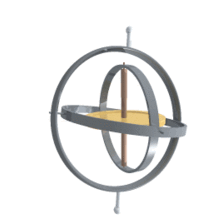
\includegraphics[width=5cm]{Images/gimbal.png}
\end{frame}

\begin{frame}
  \frametitle{Gimbal Lock}
  \centering
  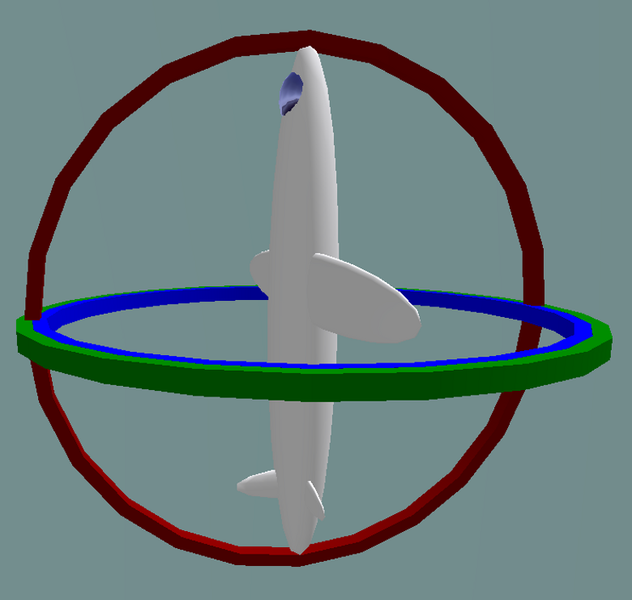
\includegraphics[width=5cm]{Images/gimbal_lock.png}
  \begin{itemize}
    \item Only 2 degrees of freedom
    \item Quaternions do not have this problem
  \end{itemize}
\end{frame}


\begin{frame}
  \frametitle{Applications: Animation}
  Problem: Smoothly animate object about arbitrary axis by arbitrary angle \pause
  \begin{itemize}
    \item Euler angles?
    \begin{itemize}
      \item Jerky  \pause
    \end{itemize}
    \item Quaternions? 
    \begin{itemize}
      \item Requires interpolation
    \end{itemize}
  \end{itemize}
  
\end{frame}

\begin{frame}
  \frametitle{Spherical Interpolation (\textit{slerp})}
  \centering
  $$ Slerp(p_0, p_1, t) = \frac{sin[(1-t)\Omega]}{sin\Omega}p_0 + \frac{sin[t\Omega]}{sin\Omega}p_1 $$
  \vspace{0.3cm}
  $$ Slerp(q_0, q_1, t) = (q_1q_0^{-1})^tq_0 $$
  \begin{itemize}
    \item Produces uniform angular velocity about a rotation axis
  \end{itemize}
  
\end{frame}

\begin{frame}
  \centering
  \huge
  Demonstration
\end{frame}

\begin{frame}
  \centering
  \huge
  Questions
\end{frame}
\end{document}
